\part{Branching}
\frame{\partpage}

\begin{frame}{Forking vs branching}
    \begin{itemize}
        \item Both represent a set of changes based on, but separate from,
            the repository's ``main'' set of commits \pause
        \item A \textbf{fork} is a completely separate repository \pause
        \item A \textbf{branch} exists within the same repository \pause
        \item Which to use? \pause
            \begin{itemize}
                \item We recommend you use branches ---
                    they are easier to work with, and keep everything within the same repository \pause
                \item In industry, many (larger) teams use forks, but also many do not
            \end{itemize}
    \end{itemize}
\end{frame}

\begin{frame}{Branching}
    \begin{itemize}
        \item Every repository starts with one branch called \texttt{master} \pause
        \item New branches can be created at any time \pause
        \item Branches can be \textbf{merged} \pause
            \begin{itemize}
                \item ``Merge A into B'':
                    take the commits (remember: changes) from branch A, and apply them to branch B
            \end{itemize}
    \end{itemize}
\end{frame}

\begin{frame}{The golden rule}
    \begin{itemize}
        \item The \texttt{master} branch should always be \textbf{deployable} \pause
            \begin{itemize}
                \item No half-finished features \pause
                \item No obvious bugs \pause
                \item \textbf{Definitely} no compile errors \pause
                \item If a VIP walked into the room and asked for a demo, \texttt{master} is what you'd show them
            \end{itemize}
    \end{itemize}
\end{frame}

\begin{frame}{Branching}
    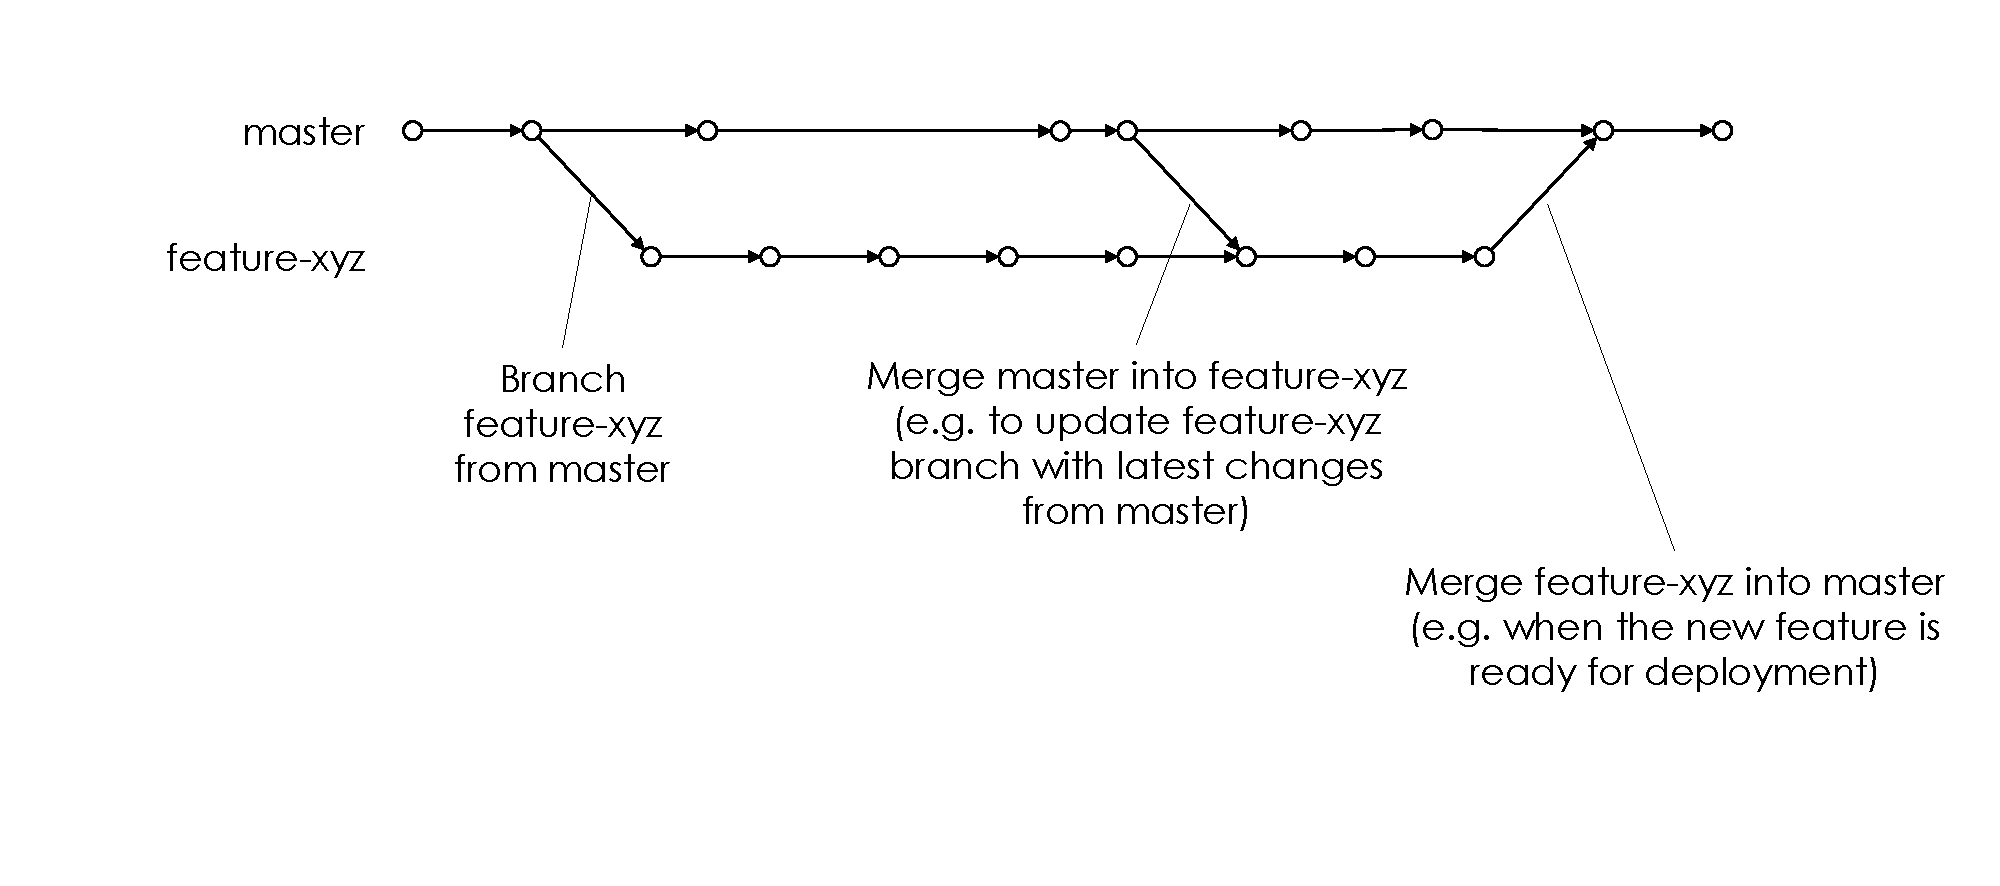
\includegraphics[width=\textwidth]{branching}
\end{frame}

\begin{frame}{Creating a branch}
    \begin{itemize}
        \item GitHub for Windows: click this button
    \end{itemize}
    \begin{center}
        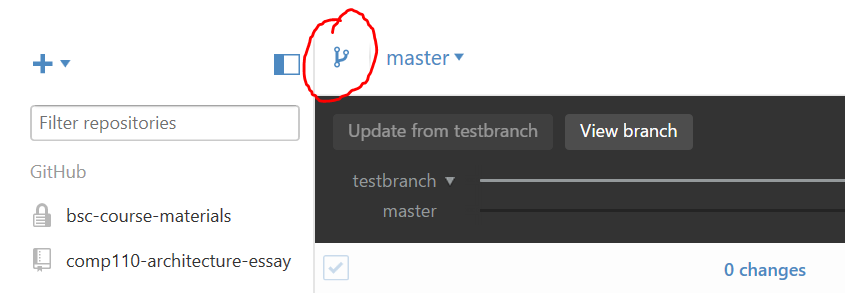
\includegraphics[width=0.7\textwidth]{github_create_branch}
    \end{center}
    \begin{itemize}
        \item TortoiseGit: use the \textbf{Create Branch} context menu item
    \end{itemize}
\end{frame}

\begin{frame}{Switching branches}
    \begin{itemize}
        \item You can switch your \textbf{working copy} (source files on disk) to a different branch
            at any time \pause
        \item Always make sure you're committing to the correct branch! \pause
        \item GitHub for Windows: use this dropdown menu
    \end{itemize}
    \begin{center}
        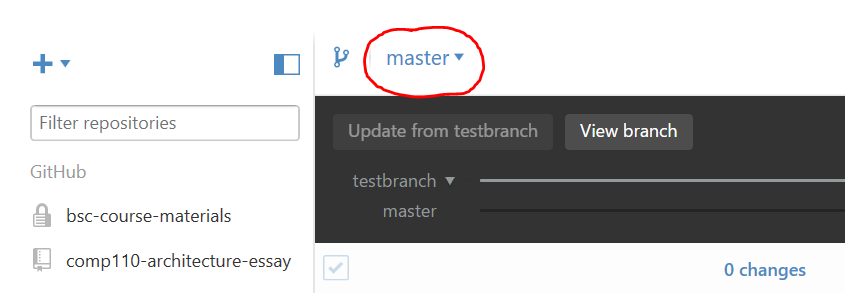
\includegraphics[width=0.7\textwidth]{github_switch_branch}
    \end{center}
    \begin{itemize}
        \item TortoiseGit: use the \textbf{Switch/Checkout} context menu item
    \end{itemize}
\end{frame}

\begin{frame}{Merging branches}
    \begin{itemize}
        \item GitHub for Windows:
            \begin{itemize}
                \item Switch to the branch you want to merge \textbf{to}
                \item Click \textbf{Compare} and select the branch you want to merge \textbf{from}
                \item Click the \textbf{Update from $\langle$branchname$\rangle$} button
                \item Resolve any conflicts
            \end{itemize}
        \item TortoiseGit:
            \begin{itemize}
                \item Switch to the branch you want to merge \textbf{to}
                \item Use the \textbf{Merge} context menu item
                \item Resolve any conflicts
            \end{itemize}
    \end{itemize}
\end{frame}

\part{Working with branches}
\frame{\partpage}

\begin{frame}{GitHub flow}
    \begin{center}
        \url{https://guides.github.com/introduction/flow/}
    \end{center}
\end{frame}

{
\setbeamercolor{background canvas}{bg=}
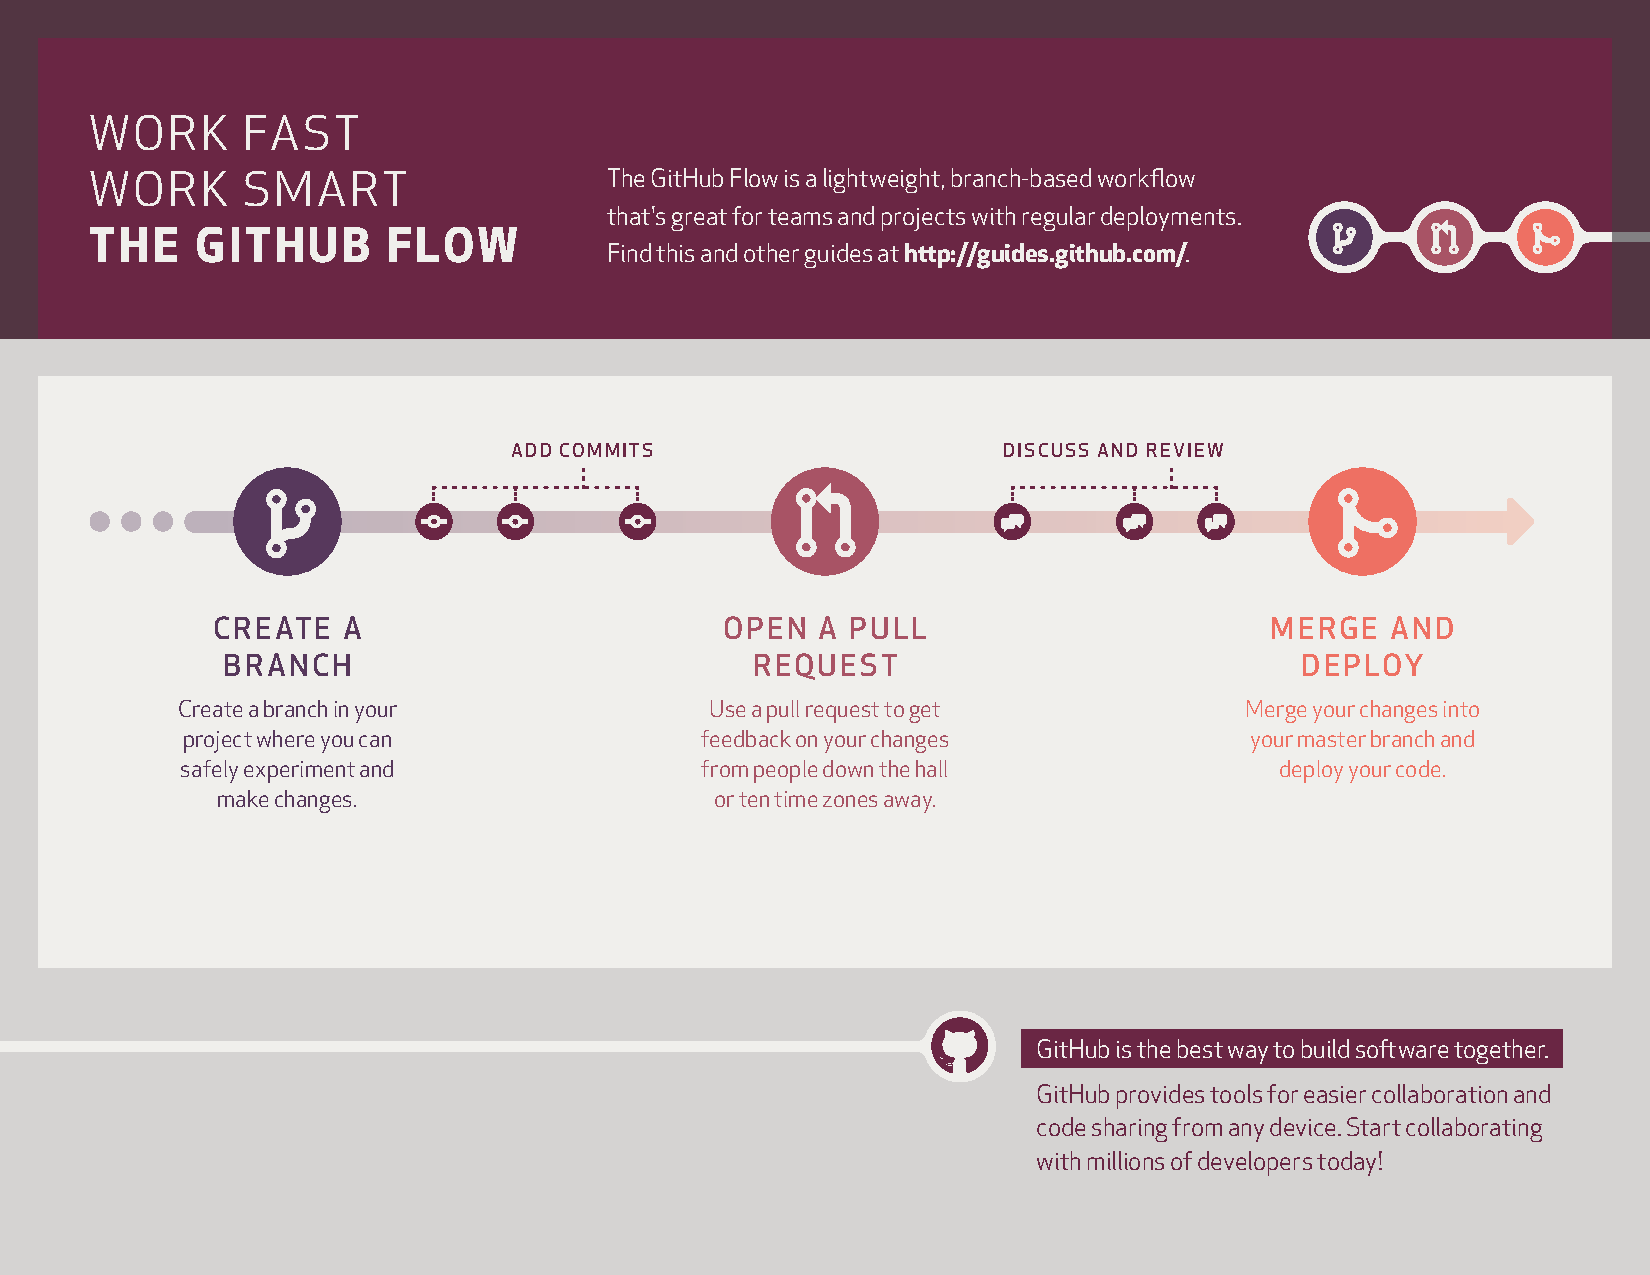
\includepdf{githubflow-online.pdf}
}

\begin{frame}{Git flow}
    \begin{center}
        \url{http://nvie.com/posts/a-successful-git-branching-model/}
    \end{center}
\end{frame}

\begin{frame}
    \begin{tikzpicture}[remember picture, overlay]
        \node[anchor=north, yshift=0.5cm] at (current page.north) {%
            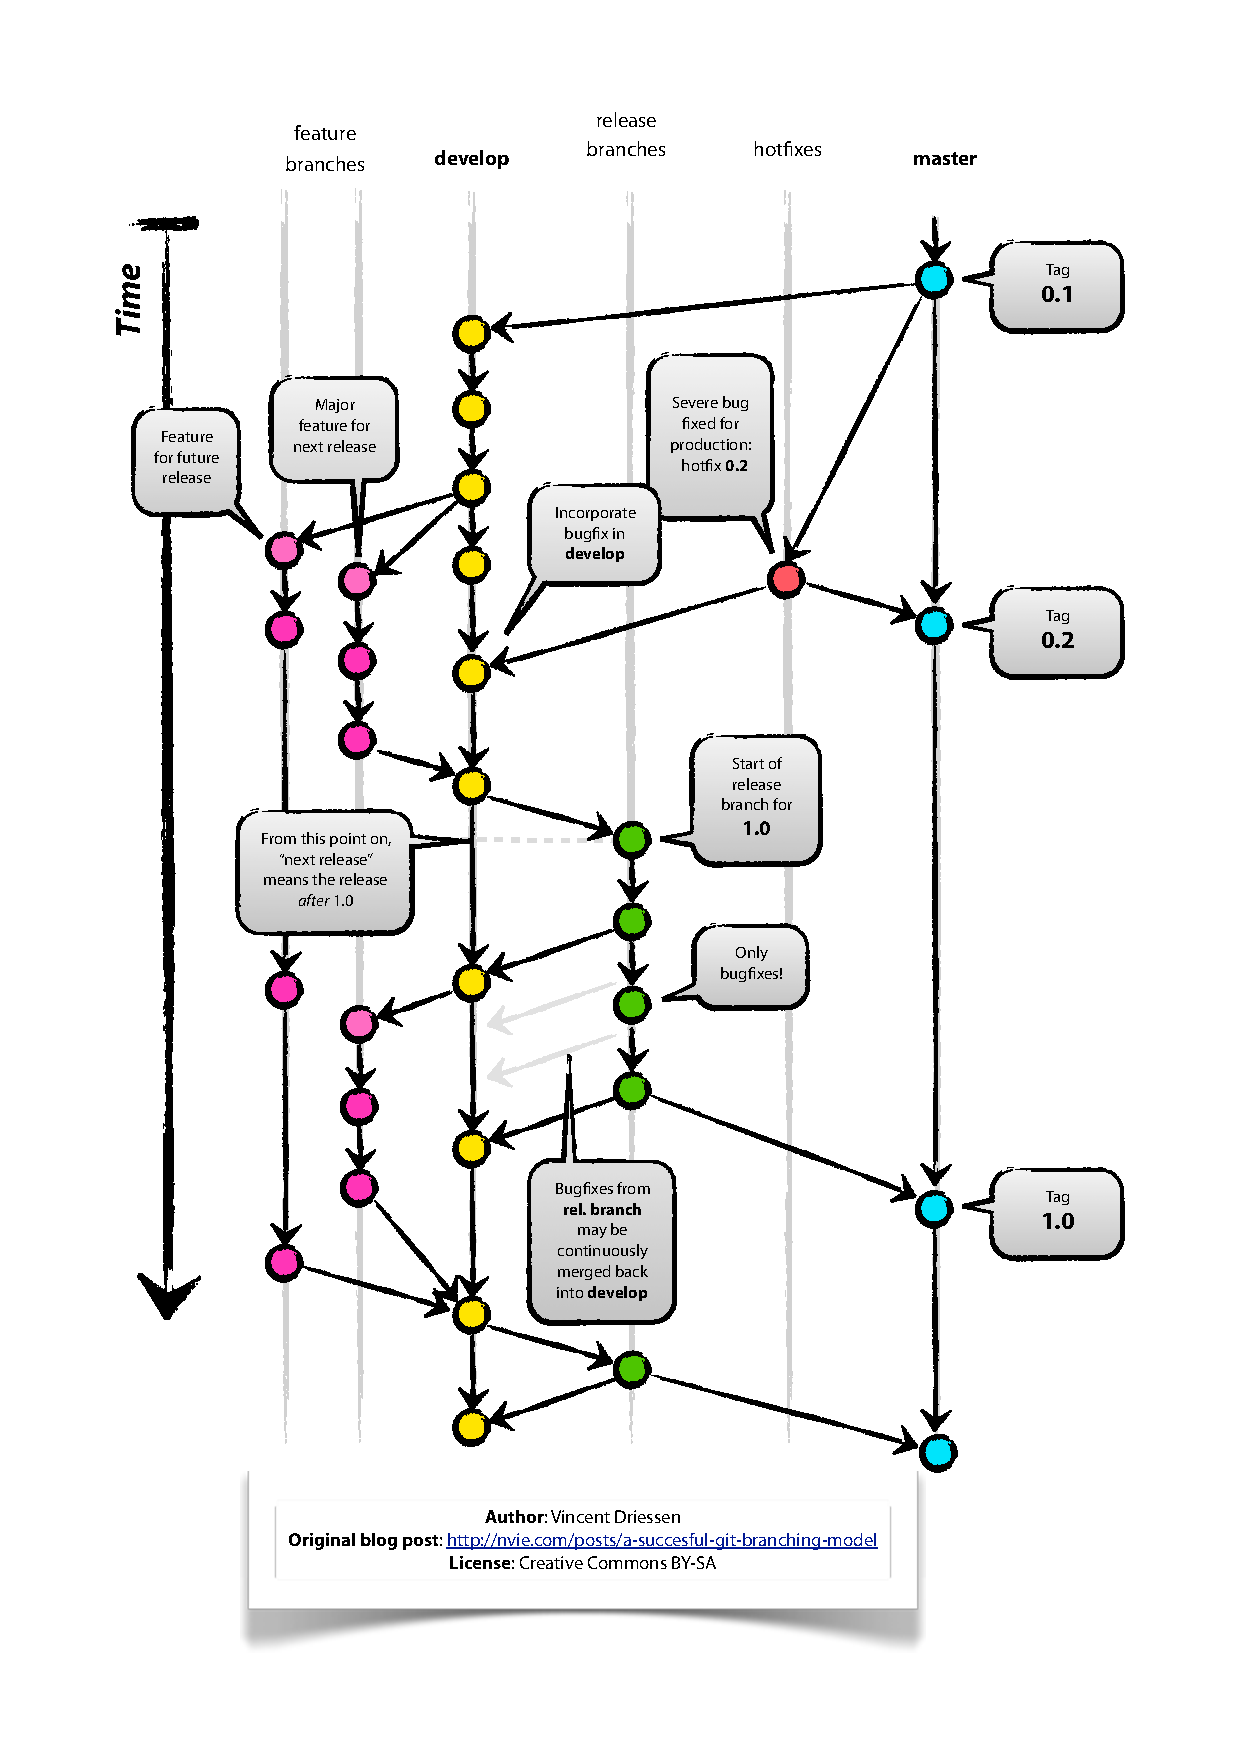
\includegraphics[height=1.1\paperheight]{Git-branching-model}%
        };
    \end{tikzpicture}
\end{frame}

\begin{frame}{Discussion}
    \begin{center}
        What are the pros and cons of \textbf{Git flow} vs \textbf{GitHub flow}?
    \end{center}
\end{frame}


